\documentclass[letterpaper,10pt,serif, draftclsnofoot,onecolumn, compsoc, titlepage]{IEEEtran}

\usepackage{graphicx}
\usepackage{amssymb}
\usepackage{amsmath}
\usepackage{amsthm}

\usepackage{alltt}
\usepackage{float}
\usepackage{color}
\usepackage{url}

\usepackage{balance}
\usepackage[TABBOTCAP, tight]{subfigure}
\usepackage{enumitem}
\usepackage{pstricks, pst-node}

\usepackage{geometry}
\geometry{margin=.75in}

\usepackage{hyperref}

% This method for displaying a relational schema was found on Stack Exchange from user Bruno Vandekerkhove
% tex.stackexchange.com/questions/296948/creating-a-relational-database-schema
\usepackage{tikz}
\usetikzlibrary{shapes, positioning, calc}
\colorlet{lightgray}{gray!20}

\usepackage{caption}

\begin{document}

% Adding these from the template in Annex C of the standard
% Some may not apply, but I'm sure most will
\section{Kyle- Database Management}
\subsection{Database organization}
The database will be organized around the core elements of surveys, questions, and responders.
These will compromise the three core tables in the database, with other tables functioning as relationships or specializations of these core tables.
All tables contain unique IDs as their primary key, and each ID is a non-negative integer.

The Survey table will contain the survey\_id as its primary key to identify each individual Survey.
Each Survey will also contain a string attribute for the title.

The Question table represents any individual kind of question.
It's attributes include a unique question\_id to serve as its primary key and the question's text as a string attribute.
The question text will be generated through the survey generation process and be stored here when the Question is created.

Surveys and Questions have a many-to-many relationship: Questions can exist in many different Surveys and Surveys contain many different questions.
To create this relationship in our database, a Contains table will exist.
The Contains table's primary key will be a combination of a survey\_id and a question\_id to correspond a questions use in a survey.
The question\_id and survey\_id individually can be used in other Contains entries, but since surveys don't have the same question multiple times, the combination will be unique for each table entry.

The Responder table will store information on the individual responders.
This includes a unique responder\_id for the primary key, two string attributes for first\_name and last\_name, the birthdate as a date attribute, and a non-negative integer attribute for the age derived from the birthdate and the current date.
The age can be updated or refreshed when necessary.
The Responder table has two specializations: a Student and a Parent.
A Parent does not contain any extra information, but a Student contains a parent1\_id and a parent2\_id to correspond to both of its parents.
The specialization is to allow for more accurate and specified queries of students and parents separately or together.
As specializations, they also contain a matching responder\_id to their corresponding Responder table entry.

To save responses, a Response table will exist.
This functions as the many-to-many relationship between Responders and Questions, but also stores the answer provided for the question.
The Response table has three specializations for each of the possible types of questions: Multiple\_Choice, Matrix, and Text.
Multiple\_Choice entries contain a character attribute for the answer, Matrix entries use a non-negative integer attribute, and Text entries use a string attribute.
Each of these specializations also contain the response\_id for the corresponding entry.

The below diagram outlines the relational database schema described above.

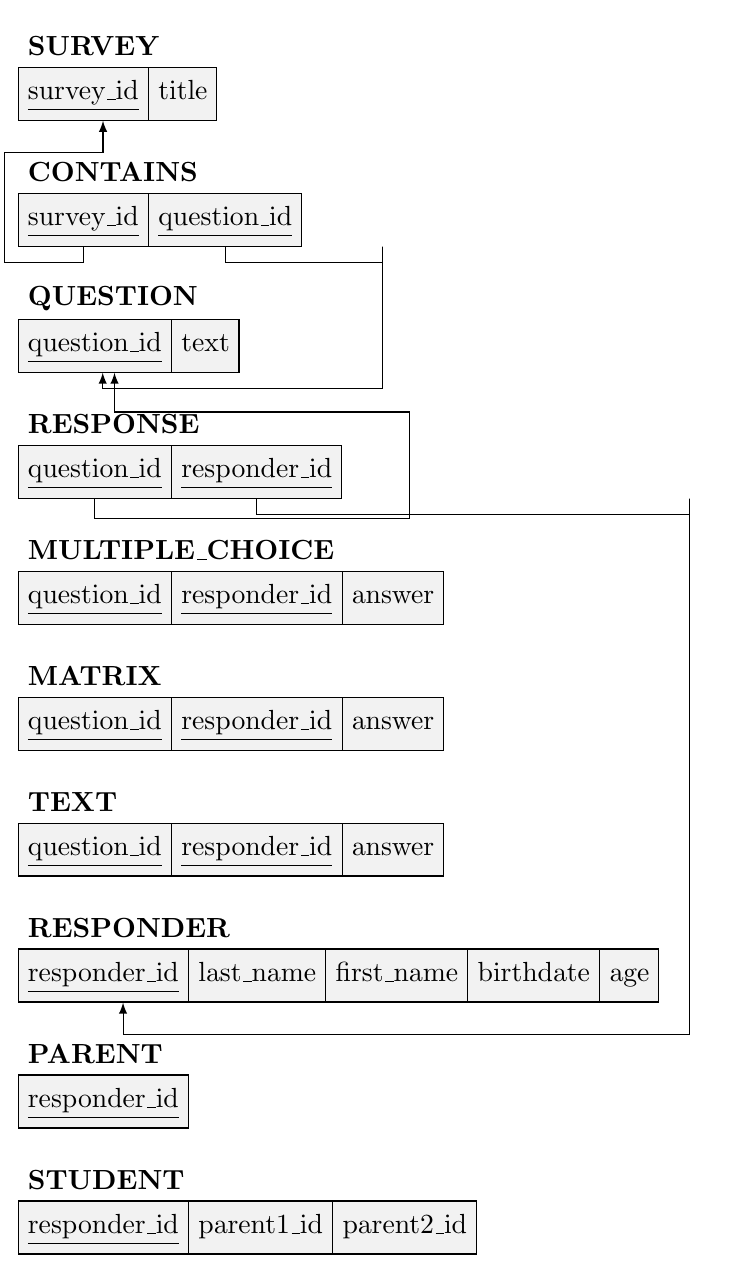
\begin{tikzpicture}[relation/.style={rectangle split, rectangle split parts=#1, rectangle split part align=base, draw, anchor=center, align=center, text height=3mm, text centered}]\hspace*{-0.3cm}

% Relations

\node (surveytitle) {\textbf{SURVEY}};
\node [relation=2, rectangle split horizontal, rectangle split part fill={lightgray!50}, anchor=north west, below=0.6cm of surveytitle.west, anchor=west] (survey)
{\underline{survey\_id}%
\nodepart{two}		title};

\node [below=1cm of survey.west, anchor=west] (containstitle) {\textbf{CONTAINS}};
\node [relation=2, rectangle split horizontal, rectangle split part fill={lightgray!50}, anchor=north west, below=0.6cm of containstitle.west, anchor=west] (contains)
{\underline{survey\_id}
\nodepart{two}	\underline{question\_id}};

\node [below=1cm of contains.west, anchor=west] (questiontitle) {\textbf{QUESTION}};
\node [relation=2, rectangle split horizontal, rectangle split part fill={lightgray!50}, anchor=north west, below=0.6cm of questiontitle.west, anchor=west] (question)
{\underline{question\_id}%
\nodepart{two}		text};

\node [below=1cm of question.west, anchor=west] (responsetitle) {\textbf{RESPONSE}};
\node [relation=2, rectangle split horizontal, rectangle split part fill={lightgray!50}, anchor=north west, below=0.6cm of responsetitle.west, anchor=west] (response)
{\underline{question\_id}%
\nodepart{two}		\underline{responder\_id}};

\node [below=1cm of response.west, anchor=west] (multiplechoicetitle) {\textbf{MULTIPLE\_CHOICE}};
\node [relation=3, rectangle split horizontal, rectangle split part fill={lightgray!50}, anchor=north west, below=0.6cm of multiplechoicetitle.west, anchor=west] (multiplechoice)
{\underline{question\_id}%
\nodepart{two}		\underline{responder\_id}
\nodepart{three}	answer};

\node [below=1cm of multiplechoice.west, anchor=west] (matrixtitle) {\textbf{MATRIX}};
\node [relation=3, rectangle split horizontal, rectangle split part fill={lightgray!50}, anchor=north west, below=0.6cm of matrixtitle.west, anchor=west] (matrix)
{\underline{question\_id}%
\nodepart{two}		\underline{responder\_id}
\nodepart{three}	answer};

\node [below=1cm of matrix.west, anchor=west] (texttitle) {\textbf{TEXT}};
\node [relation=3, rectangle split horizontal, rectangle split part fill={lightgray!50}, anchor=north west, below=0.6cm of texttitle.west, anchor=west] (text)
{\underline{question\_id}%
\nodepart{two}		\underline{responder\_id}
\nodepart{three}	answer};

\node [below=1cm of text.west, anchor=west] (respondertitle) {\textbf{RESPONDER}};
\node [relation=5, rectangle split horizontal, rectangle split part fill={lightgray!50}, anchor=north west, below=0.6cm of respondertitle.west, anchor=west] (responder)
{\underline{responder\_id}%
\nodepart{two}		last\_name
\nodepart{three}	first\_name
\nodepart{four}	birthdate
\nodepart{five}		age};

\node [below=1cm of responder.west, anchor=west] (parenttitle) {\textbf{PARENT}};
\node [relation=1, rectangle split horizontal, rectangle split part fill={lightgray!50}, anchor=north west, below=0.6cm of parenttitle.west, anchor=west] (parent)
{\underline{responder\_id}};

\node [below=1cm of parent.west, anchor=west] (studenttitle) {\textbf{STUDENT}};
\node [relation=3, rectangle split horizontal, rectangle split part fill={lightgray!50}, anchor=north west, below=0.6cm of studenttitle.west, anchor=west] (student)
{\underline{responder\_id}%
\nodepart{two}		parent1\_id
\nodepart{three}	parent2\_id};

% Foreign keys

\draw[-latex] (contains.one south) -- ++(0,-0.2) -| ($(contains.one south) + (-1,0)$) |- ($(survey.one south) + (0.25,-0.40)$) -| ($(survey.one south) + (0.25,0)$);

\draw[-latex] (contains.two south) -- ++(0,-0.2) -| ($(contains.two south) + (2,0)$) |- ($(question.one south) + (0.25,-0.20)$) -| ($(question.one south) + (0.10,0)$);

\draw[-latex] (response.one south) -- ++(0,-0.25) -| ($(response.one south) + (4,0)$) |- ($(question.one south) + (0.25,-0.50)$) -| ($(question.one south) + (0.25,0)$);

\draw[-latex] (response.two south) -- ++(0,-0.2) -| ($(response.two south) + (5.50,0)$) |- ($(responder.one south) + (0.25,-0.40)$) -| ($(responder.one south) + (0.25,0)$);

\end{tikzpicture}
\captionof{figure}{The relational database schema}

\end{document}